%--------------------------%
\section{January 2020} %---%
%--------------------------%

%%%%%%%%%%%%%%%%%%%%%%%%%%%%%%%%%%%%%
\subsection*{Classical Mechanics} %%%
%%%%%%%%%%%%%%%%%%%%%%%%%%%%%%%%%%%%%
\addcontentsline{toc}{subsection}{Classical Mechanics}

\prob{1.1}{

In figure below, a solid brass ball of mass $m$ will roll smoothly along a loop track when released from rest along a straight section.
The circular loop has a radius $R$, and the ball has a radius $r \ll R$.
What is $h$ if the ball is on the verge of leaving the track when it reaches the top of the loop?

\begin{center}
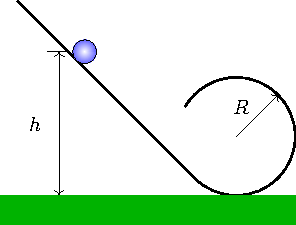
\includegraphics{January2020/1-1.pdf}
\end{center}

}

\sol{}


\prob{1.2}{

A particle is constrained to move in one dimension along the $x$ axis.
Its potential energy is given by
\begin{align*}
    U = U_0 - \frac{a x^2}{2}
,\end{align*}
where $U_0$ and $a$ are positive constants.
The particle experiences a frictional force linearly proportional to its velocity $F = -2b\dot{x}$, where $b > 0$ is a constant.
At time $t = 0$, the particle has position $x_0$ and zero velocity.

\begin{parts}
    \item Find the particle's position at a later time $t$.

    \item Find the limiting behavior of particle's position as $t \rightarrow \infty$.
\end{parts}

}

\sol{}


\prob{1.3}{

Two equal masses $m$, connected by a massless and inextensible string, hang over two pulleys (of negligible size), as shown in the figure below.
The left one moves in a vertical line, but the right one is free to swing back and forth in the plane of the masses and pulleys.

\begin{parts}
    \item Use the generalized coordinates shown in the figure, and obtaine the Lagrangian.

    \item Derive the equations of motion.

    \item Obtain the frequency of small oscillations for this system.
\end{parts}

\begin{center}
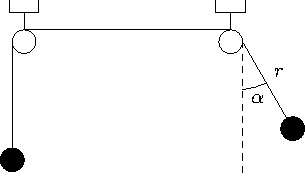
\includegraphics{January2020/1-3.pdf}
\end{center}

}

\sol{}


\prob{1.4}{

A disc of radius $R$ and mass $M$ has a hole of radius $r$.
The hole is spaced by the distance $h < R - r$ from the center of the disc as shown in the figure below.
The disc can rotate about the suspension point $O$ in the $xy$-plane in a gravitational field with normal acceleration $g$ along the $y$-axis.

\begin{parts}
    \item Write down the Lagrangian of the system.

    \item Calculate the period of small oscillations of the disc.
\end{parts}

\textbf{Hint}: The moment of inertia of a disc about its center of mass is $I = MR^2 / 2$.

\begin{center}
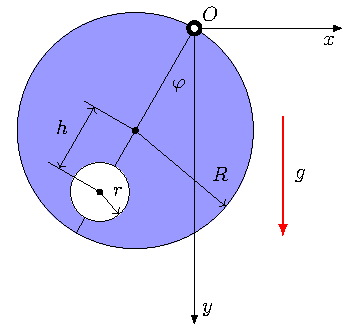
\includegraphics{January2020/1-4.pdf}
\end{center}

}

\sol{}


\prob{2.1}{

Make the (oversimplifying) assumption that the sun is a homogeneous sphere of mass $M = 0.2 \times 10^{30}~{\rm kg}$ and radius $R = 7 \times 10^{8}~{\rm m}$ with constant density.

\begin{parts}
    \item Calculate the radial pressure gradient and the pressure at the center of Sun at equilibrium.
    (You may assume that the pressure at the surface is zero).
    Compare this to the atmospheric pressure of about $10^5~{\rm N/m^2}$.

    \item Calculate the total gravitational potential energy of this mass distribution.
    Given that the sun radiates with a power of $4 \times 10^{26}~{\rm W}$, how many years would it take for the sun to lose 1/2 of the gravitational energy you calculated?

    \textbf{Note}: Newton's gravitational constant is $G = 6.674 \times 10^{-11}~{\rm N \, m^2 / kg^2}$.
\end{parts}

}

%%%%%%%%%%%%%%%%%%%%%%%%%%%%%%%%%%%%%%%%%%
\subsection*{Electricity \& Magnetism} %%%
%%%%%%%%%%%%%%%%%%%%%%%%%%%%%%%%%%%%%%%%%%
\addcontentsline{toc}{subsection}{Electricity \& Magnetism}

\prob{2.2}{

The highest-energy cosmic-rays are thought to be protons.
In principle, a cosmic-ray proton can strike a proton in a hydrogen atom in the upper atmosphere and make a $W^{+}$-boson in the process
\begin{align*}
    p + p \rightarrow p + n + W^{+}
.\end{align*}
What is the minimum energy for the cosmic-ray proton in order for this process to be allowed?
The rest masses are: $m_{\rm proton} = 938~{\rm MeV}/c^2$, $m_{\rm neutron} = 940~{\rm MeV}/c^2$, and $m_{W^+} = 80.4~{\rm GeV}/c^2$.

}

\sol{}


\prob{2.3}{

Show that the velocity-dependent potential
\begin{align*}
    U = e\phi(\vb*{r},t) - e \dot{\vb*{r}} \cdot \vb*{A}(\vb*{r},t)
\end{align*}
represents the Lorentz force $\vb*{F} = e \vb*{E} + e \vb*{v} \times \vb*{B}$ that acts on a charge $e$ moving with velocity $\vb*{v}$ in the general \textit{electrodynamic} fields $\{ \vb*{E}(\vb*{r},t), \vb*{B}(\vb*{r},t) \}$.
Here $\{ \phi,\vb*{A} \}$ are the \textit{electrodynamic potentials} that generate the fields $\{ \vb*{E}, \vb*{B} \}$ via
\begin{align*}
    \vb*{E} = -\nabla \phi - \pdv{\vb*{A}}{t}, \quad \vb*{B} = \nabla \times \vb*{A}
.\end{align*}
Show that the potentials $\phi = 0$, $\vb*{A} = t z \vu*{n}_z$ generate a field $\{ \vb*{E}, \vb*{B} \}$ that satisfies all four Maxwell equations in free space.

A particle of mass $m$ and charge $e$ moves in this field.
Find the Lagrangian of the particle in terms of Cartesian coordinates.
Show that $x$ and $y$ are cyclic coordinates and find the conserved momenta $p_x$, $p_y$.

}

\sol{}


\prob{2.4}{

Calculate the magnitude of the electric field produced by a uniform ring of total charge $q > 0$ and radius $a$ along the axis of the ring.
At what distance from the plane of the ring does the maximum value occur?

If an electron (charge $-e$ and mass $m$) is placed at the center of the ring and is then displaced by a small distance $x$ along the axis ($x \ll a$), what is its angular frequency of oscillation $\omega$?

}

\sol{}


\prob{3.1}{

Consider two conducting coaxial rings of identical radius $a$, separated by the distance $b$.
The charge on ring 1 is $Q_1$ and the charge on ring 2 is $Q_2$.
The work required to bring a point charge $q$ to the center of ring 1 is $W_1$ and to the center of ring 2 is $W_2$.

Show that the charges on the rings are
\begin{align*}
    Q_{1,2} = \frac{4 \pi \epsilon a}{b^2 q} ( a^2 + b^2 )^{1/2} \Big[ ( a^2 + b^2 )^{1/2} W_{1,2} - a W_{2,1} \Big]
.\end{align*}

}

\sol{}


\prob{3.2}{

Consider a rectangular cavity with ideally conducting walls of length $L_x$, $L_y$, and $L_z$ along the $x$, $y$, and $z$ axis, respectively.

\begin{parts}
    \item Calculate the electric field modes $E_x(\vb*{r},t)$, $E_y(\vb*{r},t)$ , and $E_z(\vb*{r},t)$ which can exist in the cavity.

    \item Calculate the resonant frequencies of the electromagnetic modes in the cavity.
    What is the minimum frequency if $L_x < L_y < L_z$?

    \item Find the relation between the amplitudes of $E_x$, $E_y$, and $E_z$.
\end{parts}

}

\sol{}


\prob{3.3}{

An uncharged metal sphere of radius $R$ is placed in an otherwise uniform electric field.

\begin{parts}
    \item Find the potential.

    \item Find the electric field in the region outside the sphere.
\end{parts}

}

%%%%%%%%%%%%%%%%%%%%%%%%%%%%%%%%%%%
\subsection*{Quantum Mechanics} %%%
%%%%%%%%%%%%%%%%%%%%%%%%%%%%%%%%%%%
\addcontentsline{toc}{subsection}{Quantum Mechanics}


\prob{3.4}{

A quantum system of Hamiltonian $H$ has a complete set of eigenstates $\ket{u_n}$ with energies $E_n$.
The system is placed in a state $\ket{\Psi}$ that is not an eigenstate.

Show that the expectation value of the Hamiltonian $\bra{\Psi} H \ket{\Psi}$ always overestimates the ground state energy.

}

\sol{}


\prob{4.1}{

Consider a system of two spin-1/2 particles with Hamiltonian
\begin{align*}
    \hat{H} = A + \frac{B}{\hbar^2} \hat{\vb*{S}}_1 \vdot \hat{\vb*{S}}_2 + \frac{C}{\hbar} ( \hat{S}_{1z} + \hat{S}_{2z} )
.\end{align*}
Find eigenvalues and eigenstates of this system.

}

\sol{}


\prob{4.2}{

Consider two electrons in a one-dimensional simple harmonic oscillator potential.
One of the electrons is in the ground state, and the other is in the first excited state.

\begin{parts}
    \item Write down the singlet-spin and triplet-spin state of this system.
    How do they behave under interchange of electron 1 and electron 2?
    Write the spatial wave functions for both states.

    \item Using the expression of a position operator in terms of lowering and raising operators $\hat{a}_i$ and $\hat{a}_i^{\dagger}$, calculate the mean expectation value of the square of the distance between the two electrons, and show that this value for the triplet-spin state is 3 times larger than for the singlet-spin state.
\end{parts}

}

\sol{}


\prob{4.3}{

Let $\ket{E_1}$ and $\ket{E_2}$ be the normalized ground and first excited states of a particle constrained in $-a \leq x \leq a$, but otherwise free.
At time $t = 0$ the particle is in state $\frac{1}{\sqrt{2}} ( \ket{E_1} + \ket{E_2} )$, and the matrix element $\bra{E_1} \hat{x} \ket{E_2} = A$ is assumed known.
Here $\hat{x}$ is the position operator and $A$ is a real constant.

\begin{parts}
    \item Calculate the expectation value of $\hat{x}$ at time $t = 0$.

    \item Find the first time $t_0$ such that the expectation value of $\hat{x}$ vanishes.

    \item Calculate the expectation value of the momentum operator $\hat{p}$ at time $t_0$.
\end{parts}

}

\sol{}


\prob{4.4}{

Show that any solution $\psi(\vb*{x},t)$ of the time-dependent Schr\"{o}dinger equation for a particle in a real potential has the property that $\pdv{|\psi|^2}{t}$ is the divergence of a vector $\vb*{j}$ and satisfies continuity equation
\begin{align*}
    \pdv{|\psi|^2}{t} + \div{\vb*{j}} = 0
.\end{align*}
Calculate the current $\vb*{j}$.

}